\documentclass[12pt,a4paper]{report}

\usepackage{styles/dolgozat}

\usepackage{listings}
\usepackage{styles/cpp}
\usepackage{styles/python}
\usepackage{styles/octave}

\usepackage{hyperref}

\usepackage{tikz}
\usepackage{caption}
\usepackage{subcaption}
\usepackage[nounderscore]{syntax}
\usepackage{forest}
\usepackage[]{algorithm2e}

\begin{document}

\pagestyle{empty} %a címlapon ne legyen semmi=empty, azaz nincs fejléc és lábléc

% A Miskolci Egyetem címere
{\large
\begin{center}
\vglue 1truecm
\textbf{\huge\textsc{Thesis}}\\
\vglue 1truecm

\includegraphics[width=4.8truecm, height=4truecm]{images/me_logo.png}\\
\textbf{\textsc{Miskolci Egyetem}}
\end{center}}

\vglue 1.5truecm %függõleges helykihagyás

% A szakdolgozat címe, akár több sorban is
{\LARGE
\begin{center}
\textbf{Parser and Interpreter Development for the
Fuzzy Behavior Description Language in MATLAB/Octave}
\end{center}}

\vspace*{2.5truecm}
% A hallgató neve, évfolyam, szak(ok), a konzulens(ek) neve
{\large
\begin{center}
\begin{tabular}{c}
\textbf{Author:}\\
Balázs Nagy\\
Computer Science
\end{tabular}
\end{center}
\begin{center}
\begin{tabular}{c}
\textbf{Advisor:}\\
Dr. Tamás Tompa
\end{tabular}
\end{center}}
\vfill
% Keltezés: Hely, év
{\large
\begin{center}
\textbf{\textsc{Miskolc, 2024}}
\end{center}}

\newpage


\newpage

\pagestyle{empty}

%Feladatkiiras
\begin{flushleft}
\textsc{\bfseries Miskolci Egyetem}\\
Gépészmérnöki és Informatikai Kar\\
Alkalmazott Matematikai Intézeti Tanszék\hspace*{4cm}\hfil \textbf{Szám:}
\end{flushleft}
\vskip 0.5cm
\begin{center}
\large\textsc{\bfseries Szakdolgozat Feladat}
\end{center}
\vskip 0.5cm
Nagy Balázs (EIO1RQ) programtervező informatikus jelölt részére.\newline

\noindent\textbf{A szakdolgozat tárgyköre:} fuzzy logika, fuzzy viselkedés, fbdl, fuzzy viselkedésleíró nyelv, fbdl fordító\newline

\noindent\textbf{A szakdolgozat címe:} Értelmező Fejlesztése a Fuzzy Viselkedésleíró Nyelvhez MATLAB és GNU/Octave Környezetben\newline

\noindent\textbf{A feladat részletezése:}

\medskip

\emph{Egy rendszer működésének a leírása különféle módokon valósulhat meg. A dolgozat ennek egy deklaratív leírási módjával, egy fuzzy szabályinterpolációs módszerre épülő automatával és annak leírónyelvével foglalkozik. A cél az, hogy MATLAB, illetve GNU/Octave nyelven is elérhető legyen egy olyan függvénykönyvtár, amely segítségével az FBDL nevű fuzzy viselkedésleírónyelvben megfogalmazott működés egyszerűen implementálhatóvá válik. A dolgozat egy rövid áttekintéssel bemutatja a fuzzy logikával kapcsolatos elméleti és a korábban elért eredményeket, majd szemlélteti az ezkre épülő leírónyelvnek a sajátosságait, annak feldolgozási módját és az automata működését. Összeveti a MATLAB és GNU/Octave implementáció módját. Konkrét példákon és szimulációkon keresztül bemutatja annak használatát.}

\medskip

%\emph{(Kisebb tagolás lehet benne, hogy jól nézzen ki.)}

\vfill

\noindent\textbf{Témavezető:} Dr. Tompa Tamás \newline

\noindent\textbf{Konzulens(ek):} Piller Imre \newline

\noindent\textbf{A feladat kiadásának ideje:}\newline

%\noindent\textbf{A feladat beadásának határideje:}

\vskip 2cm

\hbox to \hsize{\hfil{\hbox to 6cm {\dotfill}\hbox to 1cm{}}}

\hbox to \hsize{\hfil\hbox to 3cm {szakfelelős}\hbox to 2cm{}}

\newpage

\vspace*{1cm}  
\begin{center}
\large\textsc{\bfseries Eredetiségi Nyilatkozat}
\end{center}
\vspace*{2cm}  

Alulírott \textbf{Szakdolgozó Neve}; Neptun-kód: \texttt{N3P7UN} a Miskolci Egyetem Gépészmérnöki és Informatikai Karának végzős Programtervező informatikus szakos hallgatója ezennel büntetőjogi és fegyelmi felelősségem tudatában nyilatkozom és aláírásommal igazolom, hogy \textit{Szakdolgozat Címe}
című szakdolgozatom saját, önálló munkám; az abban hivatkozott szakirodalom
felhasználása a forráskezelés szabályai szerint történt.\\

Tudomásul veszem, hogy szakdolgozat esetén plágiumnak számít:
\begin{itemize}
\item szószerinti idézet közlése idézőjel és hivatkozás megjelölése nélkül;
\item tartalmi idézet hivatkozás megjelölése nélkül;
\item más publikált gondolatainak saját gondolatként való feltüntetése.
\end{itemize}

Alulírott kijelentem, hogy a plágium fogalmát megismertem, és tudomásul veszem, hogy
plágium esetén szakdolgozatom visszautasításra kerül.

\vspace*{3cm}

\noindent Miskolc, \hbox to 2cm{\dotfill} .év \hbox to 2cm{\dotfill} .hó \hbox to 2cm{\dotfill} .nap

\vspace*{3cm}

\hspace*{8cm}\begin{tabular}{c}
\hbox to 6cm{\dotfill}\\
Hallgató
\end{tabular}



\newpage

\noindent 1.

\begin{tabular}{cl}
&szükséges (módosítás külön lapon) \\
A szakdolgozat feladat módosítása& \\
& nem szükséges\\
&\\
\hbox to 4cm{\dotfill}&\multicolumn{1}{c}{\hbox to 5cm{\dotfill}}\\
dátum& \multicolumn{1}{c}{témavezető(k)}
\end{tabular}
\vskip1.5mm

\noindent 2. A feladat kidolgozását ellenőriztem:

\vskip1.5mm

\begin{tabular}{l@{\hspace*{4cm}}l}
témavezető (dátum, aláírás):& konzulens (dátum, aláírás):\\
\dotfill&\dotfill\\
\dotfill&\dotfill\\
\dotfill&\dotfill
\end{tabular}

\vskip1.5mm

\noindent 3. A szakdolgozat beadható:

\vskip1.5mm

\begin{tabular}{@{\hspace*{1.3cm}}c@{\hspace*{2.1cm}}c}
\hbox to 4cm{\dotfill}&\multicolumn{1}{c}{\hbox to 5cm{\dotfill}}\\
dátum& \multicolumn{1}{c}{témavezető(k)}
\end{tabular}

\vskip1.5mm

\noindent 4.
\begin{tabular}[t]{@{}l@{\hspace*{1mm}}l@{\hspace*{1mm}}l@{}}
A szakdolgozat& \hbox to 3.5cm{\dotfill} &szövegoldalt\\
              & \hbox to 3.5cm{\dotfill} &program protokollt (listát, felhasználói leírást)\\
              &\hbox to 3.5cm{\dotfill}   &elektronikus adathordozót (részletezve)\\
              &\hbox to 3.5cm{\dotfill} & \\
              &\hbox to 3.5cm{\dotfill} &egyéb mellékletet (részletezve)\\
              &\hbox to 3.5cm{\dotfill} &\\
\end{tabular}
\newline tartalmaz.

\vskip1.5mm

\begin{tabular}{@{\hspace*{1.3cm}}c@{\hspace*{2.1cm}}c}
\hbox to 4cm{\dotfill}&\multicolumn{1}{c}{\hbox to 5cm{\dotfill}}\\
dátum& \multicolumn{1}{c}{témavezető(k)}
\end{tabular}

\noindent 5.

\begin{tabular}{ll}
&bocsátható\\
A szakdolgozat bírálatra& \\
& nem bocsátható\\
\end{tabular}

\vskip1.5mm

\noindent A bíráló neve: \hbox to 8cm{\dotfill}

\vskip4mm

\begin{tabular}{@{\hspace*{1.3cm}}c@{\hspace*{2.1cm}}c}
\hbox to 4cm{\dotfill}&\multicolumn{1}{c}{\hbox to 5cm{\dotfill}}\\
dátum& \multicolumn{1}{c}{szakfelelős}
\end{tabular}

\noindent 6.
\begin{tabular}[t]{@{}l@{\hspace*{1mm}}l@{\hspace*{1mm}}l@{}}
A szakdolgozat osztályzata& &\\
&a témavezető javaslata:& \hbox to 3cm{\dotfill}\\
&a bíráló javaslata:& \hbox to 3cm{\dotfill}\\
&a szakdolgozat végleges eredménye:& \hbox to 3cm{\dotfill}
\end{tabular}

\vspace*{4mm}

\noindent Miskolc, \hbox to 4.5cm{\dotfill} \hspace*{2.5cm}
\begin{tabular}[t]{cc}
\hbox to 6cm{\dotfill}\\
a Záróvizsga Bizottság Elnöke
\end{tabular}


\cleardoublepage
\pagenumbering{gobble}
\tableofcontents
\cleardoublepage
\pagenumbering{arabic}

\newpage

\pagestyle{fancy}

\Chapter{Introduction}

Presented in this work is an interpreter library/package for the Fuzzy Behavior Description Language (FBDL) implemented in the Octave programming language.

This initial description of the problem at hand can either be informative or utterly confusing for anyone reading it for the first time, simply because it entails many concepts perhaps still unknown to the reader. But it is quintessential to state the main topic being tackled as to not lose sight of it amidst the following discussions that will eventually lead up to the task itself. Anyone with a moderate to advanced knowledge in the field of programming can easily comprehend the workings of an interpreter if described properly, however simply showcasing that without any prior introduction to the underlying principles would still leave a fairly large gap in the reader's mind concerning the motivation behind such a language and also its use of a myriad of fuzzy logic related ideas. Therefore it is necessary to treat the subject as a whole and describe not only the technical implementations and results, but the theory as well, on which all of it is built.

With this in mind the work is split into two main sections along with this preceding foreword to allow for some clarifications and provide a greater description of the whole subject matter. The first half exposes the reader to core concepts related to fuzzy logic and slowly builds them up into its more complex and intricate applications. Also in this part the idea of behavior control and fuzzy state machines are presented along with various mathematical models to help with formalization; it concludes with the specifications of the aforementioned Fuzzy Behavior Description Language. The second half of the work delves into the implementation and inner workings of the interpreter. In the beginning, decisions regarding language specific implementation and other architectural considerations are discussed; possible alternatives are slightly touched upon. Following a general overview of the process of interpreting a language each stage and their operations are shown separately in detail along with possible corner cases that may require special attention and samples of unit tests to check the integrity and correct operation of the program. Finally the reader is provided with working examples of source code written in FBDL and also a demonstration of said code where the output of the interpreter can be verified.

The main difficulty lies in connecting the different parts of the overarching subject, so as to allow the reader to indulge in this work without getting lost consider the following short explanation as a guide to the various topics about to be presented.

The motivation behind creating a programming language, be it any kind, is always attributed to the existence of a specific problem it is trying to solve. This could range from low-level hardware management, such as those found in embedded systems, all the way to server-side applications and numerical analysis.

The language (FBDL) appearing in this work has been constructed to serve a particular application of fuzzy logic, namely that of behavior control. For example when a system, due to some event, reacts or behaves in a certain way based on predefined rules dictating its appropriate response. A fundamental property of fuzzy logic, essentially the fact that it is continuous, make it a prime candidate for such a use, since natural systems are hard, sometimes nigh impossible to accurately model with Boolean-logic.

Describing how such a system would operate, the rules it would follow and the actions it would take can be tricky to model with ordinary programming languages. Therefore an easier alternative was designed with the primary aim of facilitating the ease of use, particularly even if the user happens to lack any kind of previous formal experience in the field of programming. To further simplify the task of using this language it takes another useful property of fuzzy logic that arises from its continuity: we are able to describe the state of a fuzzy variable or in other words the degree to which it satisfies a certain statement with the help of natural language in contrast to using concrete numerical values.

There exits many applications for fuzzy logic and its extensions, some requiring complex calculations and methods that are quite conveniently present in scientific programming languages such as MATLAB and Octave. For this reason an interpreter library in these languages would provide great utility for programs already using fuzzy logic and open new opportunities for those seeking to venture into such areas.

These ideas constitute the majority of the work, so they shall be further examined at length in the following sections.

\Chapter{Core Concepts and Previous Research}

\Section{Fuzzy Logic}
In order to gain a sound understanding of the idea of \textit{fuzziness} we must first familiarize ourselves with the notion of fuzzy sets. The concept was first introduced and described by mathematician Lotfi A. Zadeh in 1965 as an extension to classical sets. The key difference between ordinary sets and fuzzy ones is simple: In the case of the former all elements are either a part of a set or not, where as in the world of fuzzy sets an element may belong to multiple sets. The measure of how much an element is part of a given set is referred to as its \textit{degree of membership} and is calculated with the aid of the \textit{membership function}.

\SubSection{Fuzzy Set}
As opposed to classical sets, every element in a fuzyz set has an additional property beside its value that being the degree to which that given element is the set. These aspects are more formally defined in the following section.

\begin{definition}
Let $U$, referred to as the \textit{universe of discourse}, be a set containing all the elements we wish to describe and define $m:U \to [0, 1]$ as a membership function. The pair $(U, m) $ forms a fuzzy set $A$ in which $\forall x \in U$ the value given by $m(x)$ is called the degree of membership of $x$. The function $m(x)$ is equivalent to $\mu_{a}(x)$.
\end{definition}

Taking the example from Claudio Moraga's \textit{Introduction to fuzzy logic} (2005) \cite{moraga2005}: given the interval $[0, 10]$ of the real line as our universe of discourse and the statement ``x is between 3 and 5'', we may represent it with the function $\mu_{3-5}:[0, 10] \to [0,1]$. Where $\mu_{3-5}(x) = 1$ if $3 \leq x \geq 5$, and $\mu_{3-5}(x) = 0$ otherwise as seen on fig1.a. This function describes the classical set $[3, 5]$. Consider now the statement ``x is near 4''. The proximity, or nearness to the number $4$ can be represented as $4-\epsilon$, given the assumption that $\epsilon$ is a sufficiently small positive real number. Values obtained by the continued subtraction of $\epsilon$ will have a decreasing \textit{``degree of nearness''} to $4$ until the value, and subsequently those smaller then itself, is no longer considered to be ``near'' the number $4$. Repeating this experiment with $4+\epsilon$ and the continued addition of $\epsilon$ will yield symmetric results. If we take the function $\mu_{near 4} : [0, 10] \to [0, 1]$ to represent this statement just as previously, it becomes apparent that it cannot be of the same kind as $\mu_{3-5}$ (that lead to a classical set). If we assume that 3 and 5 are acceptable limit points for ``near 4” and marking these as , $\alpha_{min} = 3, \alpha_{max} = 5, beta = 4$, then

\[
	\mu_{near 4}(x) =
		\begin{cases}
			0, &x \leq \alpha_{min} \text{ or } x \geq \alpha_{max}\\
			1, &x = \beta\\
			\frac{x - \alpha_{min}}{\beta - \alpha_{min}}, &\alpha_{min} < x < \beta\\
			\frac{\alpha_{max} - x}{\alpha_{max} - \beta}, &\beta < x < \alpha_{max}.\\
		\end{cases}
\]

The function will be continuous and increasing for $3 < x < 4 and$ will be continuous and decreasing for$ 4 < x < 5$. Without further information, linear transitions will be chosen as shown in fig1.b. $\mu_{near 4} $ represents a \textbf{fuzzy set}.

[figures of the previous example]
\begin{figure}[!h]
\centering
\begin{subfigure}{.5\textwidth}
	\centering
	\begin{tikzpicture}
		\draw (-3, 0) -- (3, 0);
		\draw (-3, 0) -- (-3, 3);
		\draw (-3, 3) -- (3, 3);
		\draw (3, 0) -- (3, 3);
 	\end{tikzpicture}
  	\caption{Classical set}
  	\label{fig:sub1}
\end{subfigure}%
\begin{subfigure}{.5\textwidth}
	\centering
  	\begin{tikzpicture}
		\draw (-3, 0) -- (3, 0);
		\draw (-3, 0) -- (-3, 3);
		\draw (-3, 3) -- (3, 3);
		\draw (3, 0) -- (3, 3);
	\end{tikzpicture}
  	\caption{Fuzzy set}
  	\label{fig:sub2}
\end{subfigure}
\caption{Difference in steepness during the transition from 0 to 1.}
\label{fig:steepness}
\end{figure}

Other than assigning values linearly to elements not fully contained inside a fuzzy set any kind of membership function can be utilized, but by far the most common is the previously mentioned linear way, which produces a trapeziod shape during visualization (Triangles arise, when the upper side of the trapezoid is a point). As mentioned by \cite{sabri2013}, in terms of terminology the following expressions are defined regarding any given fuzzy set:

\textit{Core:} Elements where the membership function is 1:
\[
	\text{core}(A) = \{x \in U \vert \mu_{\alpha}(x) \geq \alpha\}
\]

\textit{Support:} Elements where the membership function is greater than 0:
\[
	\text{support}(A) = \{x \in U \vert \mu_{\alpha}(x) > 0\}
\]

\textit{Boundary:} Elements where the membership function is between 0 and 1:
\[
	\text{boundary}(A) = \{x \in U \vert 0 < \mu_{\alpha}(x) < 1\}
\]

\textit{Height:} The height of the fuzzy set $A$ is the maximum value taken on by the membership function:
\[
	\text{height}(A) = \{x \in U \vert \max(\mu_{\alpha}(x))\}
\]

\SubSection{Various Membership Functions}
An example of the different shapes that a membership function may take include the following cases and their respective definitions appearing in \cite{sabri2013}:

\textbf{Triangular} (Same as in the above example, a special case of the trapezoid):
\[
	\mu_{A}(x) =
		\begin{cases}
			0, &x \leq \alpha_{min} \text{ or } x \geq \alpha_{max}\\
			1, &x = \beta\\
			\frac{x - \alpha_{min}}{\beta - \alpha_{min}}, &\alpha_{min} < x < \beta\\
			\frac{\alpha_{max} - x}{\alpha_{max} - \beta}, &\beta < x < \alpha_{max}.\\
		\end{cases}
\]

\textbf{Trapezoidal} (With the upper side (core) taking values from [$\beta_1$, $\beta_2$]):
\[
	\mu_{A}(x) =
		\begin{cases}
			0, &x \leq \alpha_{min} \text{ or } x \geq \alpha_{max}\\
			\frac{x - \alpha_{min}}{\beta_1 - \alpha_{min}}, &\alpha_{min} < x < \beta_1\\
			\frac{\alpha_{max} - x}{\alpha_{max} - \beta_2}, &\beta_2 < x < \alpha_{max}.\\
		\end{cases}
\]

\textbf{$\Gamma$-membership} function:
\[
	\mu_{A}(x) =
		\begin{cases}
			0, &x < \alpha\\
			1-e^{\gamma(x-a)^2}, &\alpha_{min} < x < \beta_1\\
		\end{cases}
\]

\textbf{S-membership} function:
\[
	\mu_{A}(x) =
		\begin{cases}
			0, &x \leq \alpha_{min} \text{ or } x \geq \alpha_{max}\\
			2 \left( \frac{x - \alpha_{min}}{\alpha_{max} - \alpha_{min}} \right) pow2, &\alpha_{min} < x < \beta\\
			1 - 2 \left( \frac{x - \alpha_{min}}{\alpha_{max} - \alpha_{min}} \right) pow2, &\beta < x < \alpha_{max}.\\
		\end{cases}
\]

\textbf{Logistic} function:
\[
	\mu_{A}(x) = \frac{1}{1 + e^{-\gamma x}}
\]

\textbf{Exponential-like} function:
\[
	\mu_{A}(x) = \frac{1}{1 + \gamma(x - \beta)^2}
\]
where $\gamma > 1$.

\textbf{Gaussian} function:
\[
	\mu_{A}(x) = e^{-\alpha (x - \beta)^2}
\]

Besides these any function that fits the intended purpose of characterizing a certain fuzzy set is acceptable and it is left up to the discretion of experts in the given field to decide which one is most appropriate.

[figures some previous functions]

\SubSection{Dealing with Multiple Fuzzy Sets}
There are some cases, where precise numerical measurements might not be required or even be detrimental, for example stating someone's age as being 17 years 32 days and 8 hours old, does not necessarily demand such accuracy. It is much more sensible to describe that person simply as young. This notion of the use of words in our statements instead of numerical values was introduced by Zadeh in 1975 and is called a \textbf{linguistic variable}. The varying values taken by such a variable can be described by \textbf{linguistic terms}, such as \textit{low, middle, high, very small, average, large}, meaning we are able to take advantage of natural language, thus making it easier to work with.

For a simple example consider one's age as a variable and the two sets: young and old. A person who is 5 years of age is considered very young and not at all old, similarly someone in their twenties may be called young, but slightly old as well, however a middle aged individual of 43 years is neither very young nor very old, but rather an even mix of both. Representing the two fuzzy sets, young and old, on fig3 we can see they overlap. Any value at this given interval of overlay is a linear combination of, in this particular case, both of these fuzzy sets. The number of sets can, of course, be extended and then the values at these intersection would be a linear combination of all the defined sets, given that they overlap. From giving proper definitions of how to operate on these linguistic variables arises the notion of \textbf{fuzzy logic} and subsequently it serves as the basis for many advanced concepts such as: inference, fuzzy decision making and fuzzy control.

[Overlapping fuzzy sets with point x demonstrating linear combination of values]
\begin{figure}[!h]
\centering
	\begin{tikzpicture}
		\draw (-3, 0) -- (3, 0);
		\draw (-3, 0) -- (-3, 3);
		\draw (-3, 3) -- (3, 3);
		\draw (3, 0) -- (3, 3);
 	\end{tikzpicture}
\end{figure}

\Section{Applications of Fuzzy Logic}
Many fields make use of fuzzy logic and all the differing unique characteristics from ordinary sets that it has to offer. Fuzzy logic is best suited for problems that may be hard to define or model precisely with Boolean-logic. A collection of some notable examples of already tried and implemented solutions explored by \cite{makkar2018} are discussed in this section.

\SubSection{Healthcare}
Due to the intrinsic non-linearity of biomedical systems it is difficult to accurately model various processes. Regulation of blood pressure in the case of medical patients has been tested with the help of a real time drug delivery system that used an integrated fuzzy controller. Separately, it has also been shown that test reports yield estimates of likelihood rather than confirmation of presence or absence of a disease, hence these empirical estimates can be treated as the output of a membership function and used as such in fuzzy inference modelling.

\SubSection{Chemical Science}
A fuzzy control system was used to both apply current to a series of anodes protecting an underground pipeline and to minimize the system's power consumption. For comparison the system used 126 \textit{fuzzy rules} (further discussed in the following chapter) and an empirically adjusted membership function to optimize the model. Another study conducted in relation to pH measurement in waste water adopted fuzzy logic to calculate errors and acceptable levels of pH in the data. 

\SubSection{Optimization Problems (Operations Research)}
Pappis and Mamdani (1977) applied fuzzy logic to control the flow of traffic at an intersection of two one-way streets and minimize traffic obstruction. Teodorovic and Kalie (1996) experimented with fuzzy logic based decisions for choosing the mode of transportation in order to minimize both the cost of traveling and the travel time. .Jarkko and Esko (2003) had applied fuzzy logic to minimize the waiting time and risk of collisions during the operation of traffic signals .

\SubSection{Behaviour Control}
Perhaps the most intriguing application found in the field of fuzzy logic is the modeling of certain behaviors of systems; most peculiar of them being ethological ones. Of course the topic being the bulk of this work, its details and methods of operation will we further elaborated, but here we examine the interesting possibilities fuzzy logic and fuzzy control can offer us in the form of  behavior control. The main difficulty of simulation or prediction of evolution regarding such systems comes from its dependence on a large number of variables and combinations of possible outcomes making it extremely difficult to model with great accuracy. Fuzzy logic allows, in a sense, to approximate these processes and provide a reasonably close solution to the problem. It closely resembles the natural ways of decision making as well, given the fact that there are no sharp boundaries needing to be crossed while considering a decision as it follows, by definition, a continuous range of values.

\Section{Fuzzy Rules}
Following \cite{sabri2013}, the behavior of a system can be represented by a simple model if we consider only its relevant aspects. Such a construct makes use of a set of rules in the ``if - then'' form. Fuzzy rules are categorized by two major types, Mamdani fuzzy rules and Takagi-Sueno fuzzy rules. In the general form of a fuzzy rule a list of antecedents is followed by a number of consequents such that:

\begin{quote}
	if $<antecedent_1>$ and $\ldots$ and $<antecedent_n>$, then
	$<consequent_1>$ and $\ldots$ and $<consequent_n>$
\end{quote}

\noindent where the \textit{antecedent} is of the form $v_1$ is $S_1$ and the consequent $z_1$ is $W_1$ respectively. $v_i$ is an input variable belonging to the input fuzzy set $S_i$ and $z_j$ is an output variable of the output fuzzy set $W_j$.
In the case of Takagi-Sueno fuzzy rules the consequents are replaced with functions of the input variables so that $z_j = f_p(v_1, \ldots, v_i)$, where $f_p$ is any real function.

\SubSection{Fuzzy Inference}
In order to use fuzzy logic for any sort of application we must first consider how to integrate it with existing Boolean-logic. More precisely, we are interested in a solution that operates on linguistic variables and an outcome that relies solely on fuzzy rules along with linguistic terms. Since the input variables to any given system are usually not fuzzy ones, they must be converted to satisfy this requirement in order to then later be used within the fuzzy application. This first step is called \textbf{fuzzification} and as the name implies we make sure to supply our further calculations with variables of the correct form. By taking the desired element $x \in U$ from our universe of discourse and some fuzzy set $A$ we convert $x$ to a membership function value, given by $\mu_{A}(x)$. Repeating this procedure for every element we wish to utilize yields a degree of membership for each one, therefore translating all discrete inputs to fuzzy ones.

Now that we have a number of fuzzy variables to work with the next step is to apply predefined rules of the form described in the previous section. This step is referred to as \textbf{inference} and mathematically it is a mapping of the antecedents (input variables) to the consequents (output variables), resulting in an output fuzzy set. A degree of membership of any variable in this resultant set is depended upon the degree of membership of values in the input set or sets that have been defined by the given rule. That is to say, let $A$ and $B$ be fuzzy set of the antecedent and $C$ of the consequent respectively and $X$, $Y$, $Z$ linguistic terms. Then, according to the rule 
	
\[
	\text{if } A \text{ is } X \text{ and } B \text{ is } Y \text{ then } C \text{ is } Z
\]
the inference process will calculate the output fuzzy set $C$ based on the known values of $\mu_A(X)$ and $\mu_B(Y)$.

In a similar manner to the calculation of the membership functions there are a multitude of methods which are applicable in determining the output, these are functions that do the actual mapping between the two sets of antecedent and consequent. This process of \textbf{fuzzy rule interpolation} (FRI) entails a great number of ways in which different aspects and characteristics of the membership functions are considered and thereafter the calculations made, each having their advantages and difficulties. Numerous techniques are listed in contemporary research with regards to FRI methods \cite{kovacsjohanyak2018}

The result, or in other words the consequent, of each rule is obtained and then all these functions are aggregated to produce a final, combined output, which is then finally converted back into crisp, non-fuzzy values in the process of \textbf{defuzzification}. The most common form of procedure employed to regain these crisp values is by taking the aforementioned combined function and finding its centroid.

\Section{Fuzzy Automaton and Behavior Control}
Behavior is, in the most simple sense, a series of states, where a transition between two states occurs in response to some event. The closest and most accurate mathematical model to this notion are state machines, which follow an almost identical definition. 

Integrating fuzzy logic into a state machine will result in a Fuzzy Finite-state Automaton (FFA); this work uses the same model as in \cite{pillerkovacs2015}; where the definition is given in the following manner:

\[
	F = (S, X \delta, P, O, Y, \sigma, \omega),
\]

\noindent where

\hspace*{0.5cm}%
\begin{minipage}{.8\textwidth}%
       $S$ is a finite set of fuzzy states, $S = \{\mu_{s1}, \mu_{s2}, \ldots, \mu_{sn}\}$.

      $X$ is a finite dimensional input vector, $X = \{x_1, x_2, \ldots, x_m\}$.

      $P \in S$ is the fuzzy start state of $F$.
      
     $O$ is a finite dimensional observation vector, $O = \{o_1, o_2, \ldots, o_p\}$.
	
	$Y$ is a finite dimensional output vector, $Y = \{y_1, y_2, \ldots, y_l\}$.
	
	$\delta : S \times X \rightarrow S$ is the fuzzy state-transition function which is used to map the current fuzzy state to the next fuzzy state based on the input value.
	
	$\sigma : O \rightarrow X$ is the input function which is used to map the observation to the input value.
	
	$\omega : S \times X \times Y$ is the output function which is used to map the fuzzy state and input to the output value.
\end{minipage}%

\begin{figure}[!h]
	\centering
	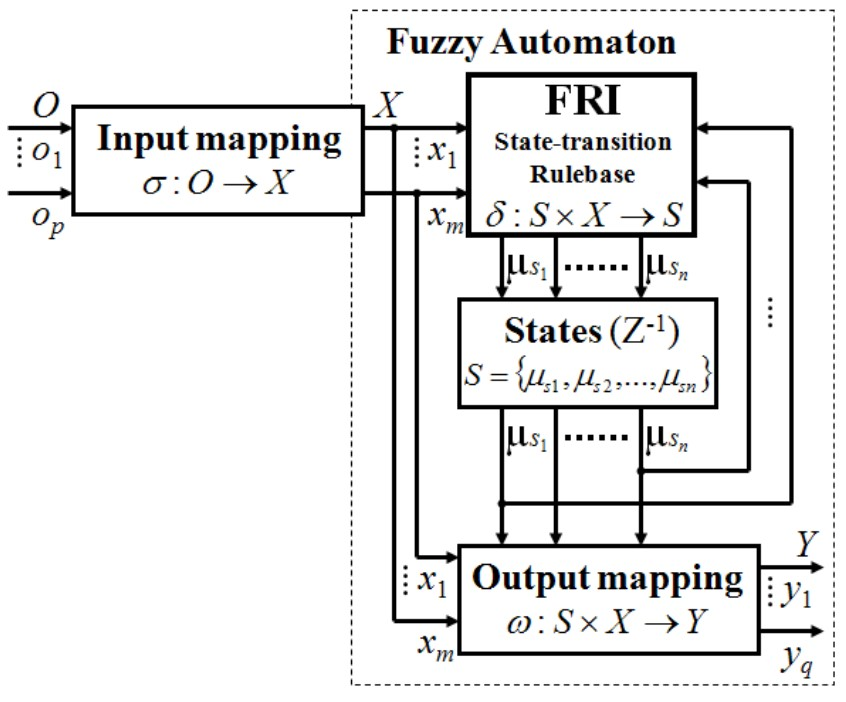
\includegraphics[width=0.6\textwidth]{images/fuzzy_automaton}
	\caption{Fuzzy Automaton}
\end{figure}

\Section{Fuzzy Behavior Description Language}
After having discussed in detail the needed prerequisites for greater understanding we can finally turn our attention to the main topic of this work, namely the language with which the aforementioned fuzzy behavior can be described. 


\SubSection{Motivation}
The language aims to provide an environment that enables the creation of programs utilizing fuzzy logic while requiring minimal to almost no prior knowledge in the field of programming. The target applications mainly entail those that delve into behavior control, as its name implies, and in order to facilitate the efficient development of such programs a higher level of abstraction is required leaving the specific implementations with regards to hardware constraints and fuzzy calculations to their respective layers of operation.

\SubSection{Language Specifications}
An easy to use language encompasses not just logical abstraction, but is also simple in terms of syntax.
An SQL-like syntax for verbosity and the lack of special characters or any complicated notation schemes makes it appeal to a wider audience than it would otherwise. The specifications for the grammar is provided below using the extended Backus-Naur form. Note that the interpreter discussed in this work is based on a JavaScript implementation from the same paper \cite{pillerkovacs2015}.

\begin{grammar}
<behavior> ::= universe+ rulebase+ [init]

<universe> ::= `universe' string [`description' string] symbol+ `end'

<symbol> ::= string number number

<rulebase> ::= `rulebase' string [`description' string] rules `end'

<rules> ::= rule+

<rule> ::= `rule' [`description' string] [`use'] string [`when' predicates] `end'

<predicates> ::= predicate (`and' predicate)*

<predicate> ::= string `is' string

<init> ::= `init' [`description' string] (string (string | number))+ `end'
\end{grammar}

For a more concise representation a railroad diagram of each element is also included \cite{pillerkovacs2015}.

\begin{figure}[!h]
	\centering
	\begin{subfigure}[b]{0.8\textwidth}
		\centering
        	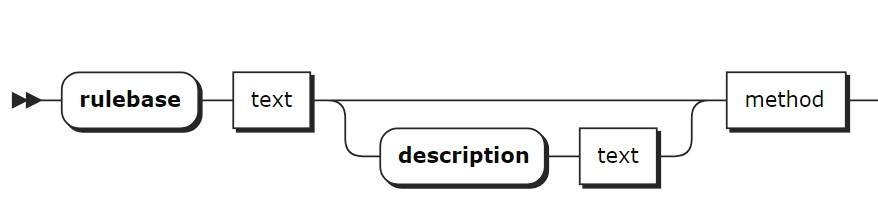
\includegraphics[width=0.8\textwidth]{images/rulebase_1}
		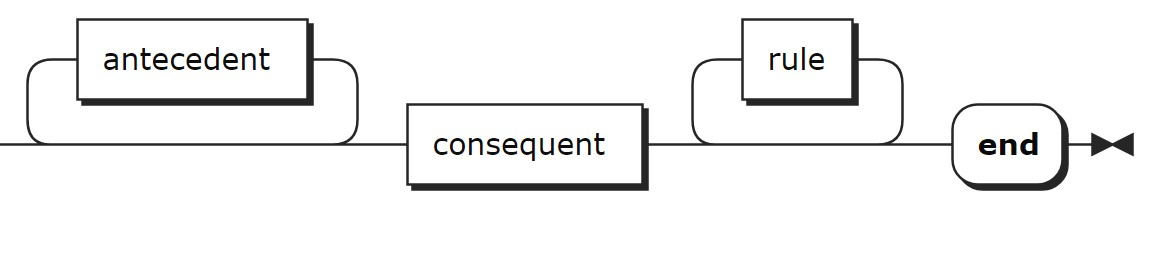
\includegraphics[width=0.8\textwidth]{images/rulebase_2}
        	\caption{Rulebase definition}
    \end{subfigure}
	
	\begin{subfigure}[b]{0.9\textwidth}
        	\centering
        	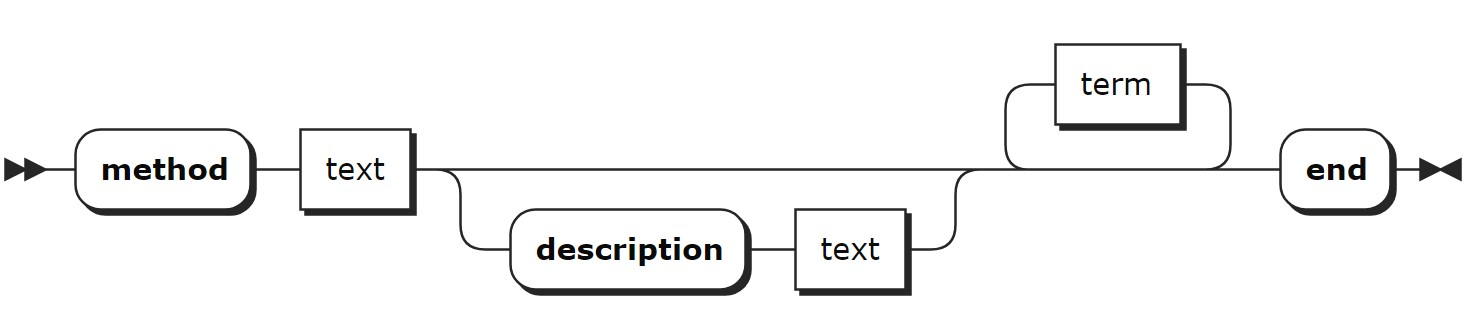
\includegraphics[width=0.8\textwidth]{images/method}
		\caption{Method definition}
    \end{subfigure}
    
    \begin{subfigure}[b]{0.9\textwidth}
        	\centering
        	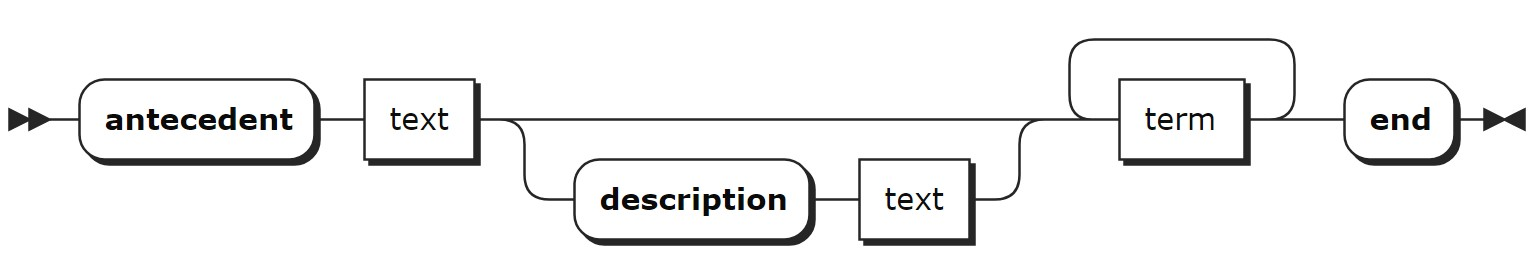
\includegraphics[width=0.8\textwidth]{images/antecedent}
		\caption{Antecedent definition}
    \end{subfigure}
    
    \begin{subfigure}[b]{0.9\textwidth}
        	\centering
        	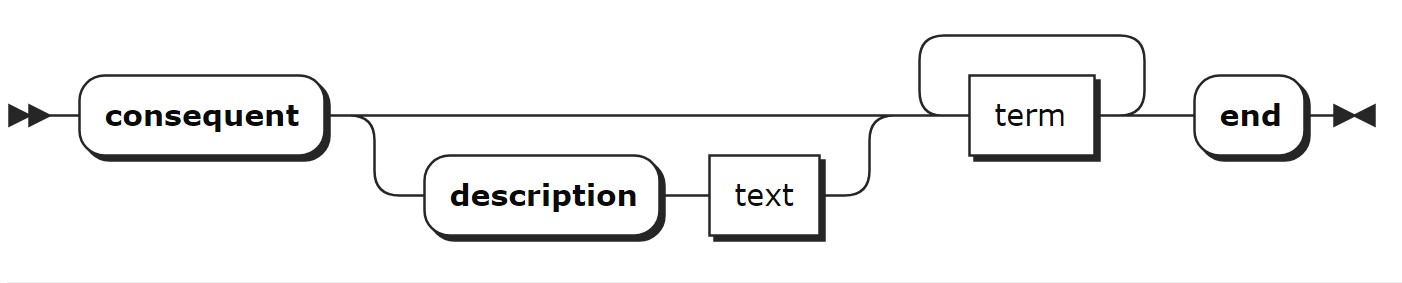
\includegraphics[width=0.8\textwidth]{images/consequent}
		\caption{Consequent definition}
    \end{subfigure}
    
	\caption{Syntax diagram of language elements}
\end{figure}

[Fix rule and term block]

\Chapter{Design}

\Section{Requirements and Technical Considerations}
Due to past research around fuzzy logic and its application in behavior control the need for having an adequate language along with a library or interpreter to make calculations easier also arose. For avoiding ambiguity, in the following discussions the words library, program and interpreter are used interchangeably and should be treated as referring to the same concept, namely the FBDL interpreter. The entire operation of the program is based on the preceding works and research in fuzzy behavior control and behavior-based systems \cite{pillerkovacs2019}.

Many of the applied examples were produced in the MATLAB language, therefore facilitating the need for  developing a framework capable of operation in that environment. The similarity between the MATLAB and Octave programming languages presented a great opportunity; implementing the interpreter in such a way as to conform to both languages would make it more accessible and allow for wider usage. Therefore the decision was made to produce a program that uses in its operation only minimal parts that are found in both languages, thus making it compatible and interoperable.

To further elaborate, the usage of language specific components and features should be kept at a minimum or avoided altogether if possible, for example the definition of classes or application of several built in functions, function definitions, unit tests etc. are such areas where the two target languages tend to differ quite majorly. It also does not help that at each iteration and new versions these differences grow ever larger since new features are added and perhaps old ones modified or removed, hence implementation with only basic and fundamental features of each language should be prioritized to the utmost extent.


\Section{Structure of The Interpreter}
The difference in function definitions, the most noticeable one being that in MATLAB scripts cannot contain any local function definitions before version R2016b, and also other incompatibilities related to the syntax of this operation are the main reason that the program is organized in a way so that every function definition occupies its own $.m$ file. 

Since the interpreter is not a standalone program, rather a library, its entry point is a function that gets called from the user of this library. From there it goes through each stage of interpreting the input; it is comprised of 3 major parts and a lot of smaller, auxiliary functions that help in completing the task, along with making the program code more readable and modular.

\begin{figure}[!h]
	\centering
	\begin{forest}
	  for tree={
	    font=\ttfamily,
	    grow'=0,
	    child anchor=west,
	    parent anchor=south,
	    anchor=west,
	    calign=first,
	    edge path={
	      \noexpand\path [draw, \forestoption{edge}]
	      (!u.south west) +(7.5pt,0) |- node[fill,inner sep=1.25pt] {} (.child anchor)\forestoption{edge label};
	    },
	    before typesetting nodes={
	      if n=1
	        {insert before={[,phantom]}}
	        {}
	    },
	    fit=band,
	    before computing xy={l=15pt},
	  }
	[Interpreter
		[main.m \textit{(Entry point)}]
		[lexer
			[utils
				[\textit{Utility programs}]
			]
		    	[getNextToken.m]
		    	[\textit{Lexical analyzer functions}]
		  ]
	 	 [parser
	    		[parer.m]
	    		[\textit{Parsing functions}]
			[\textit{Semantic checkers}]
	  	]
		[engine
	    		[text1.2.1]
	    		[text1.2.2]
	  	]
	]
	\end{forest}
	\caption{Interpreter file hierarchy}
\end{figure}

[Add figure of abstract operation, eg.: interpreter parts and data flow]


The program's entry point is a callable function that takes either a string or a file path as input and returns the solution vectors resulting from the fuzzy calculations. In both cases the content supplied must be a valid piece code written in FBDL. 

[Extend with return value and engine/state machine]
\begin{octave}
function retval = main(input, type)
  retval = 0;
  addpath("lexer");
  addpath("lexer/utils");
  addpath("parser");
  addpath("engine");

  content =  "";
  if strcmp(type, "f")
    content = fileread(input);
  elseif strcmp(type, "s")
    content = input;
  else
    % TODO: Print usage
  end

  behavior = parser(content);
  % Fuzzy state machine
  %stateMachine = createStateMachine(behavior);
  %step(stateMachine);
end
\end{octave}

Functions that facilitate the usage of the program must first be ``included'' with path definitions treating the above entry point as root, since they are stored in their separate files. Supplying the function with either type of valid input will initiate its operation, anything other than that will result in an error and the user will be provided a message on basic usage.

The function $parser()$ being called first might be a bit counter intuitive, but the lexer and parser operate simultaneously, not in a procedural manner, where the output of the lexer is the input to the parser. Of course doing it that way is also possible, returning a vector of tokens and then parsing that, however it is not just less efficient, but at the same time takes away the ability to report errors with correct positional messages, since that information is carried by the lexer and not the tokens.

The sequence of operations is perhaps best demonstrated via a simple model:

[Add pseudo code to describe functioning]

The parser continuously requests tokens from the lexer and at the same time it builds the syntax tree for the entire program, after which this completed structure is passed to the engine for calculations.

\Section{Data Structures}
Regarding the data structures used in the program, the most compatible with both languages were found to be the \textit{struct} and \textit{cell}, hence all complex objects are stored in such a manner. For clarity,  the \textit{cell} data type is not used as frequently, but in some parts it is more appropriate than other solutions. The most important of these objects is the \textit{lexer}, but others include \textit{token} and the \textit{syntax tree} along with other minor internal data structures that store and manage the information read during or after lexical analysis.

\SubSection{Lexer}
This structure holds the input and several key information about the position of the cursor currently analyzing the text. Due to organizing every function into its own file the lexer can only be either a global structure that gets modified by any given function or it is created locally in the top most function in terms of calling hierarchy and is passed around by every other function that needs either access to the input stream or the metadata stored in it. A separate function for creating a lexer is provided in foresight to unit testing, so as to avoid having to create it in every single test case.

\begin{octave}
function lexer = createLexer(content)
  keywords = {
    "universe", "rulebase", "end", "description", "rule",...
    "when", "and", "is", "init",  "use"
  };

  lexer = struct(
    "content", content,
    "content_len", length(content),
    "cursor", 1,
    "line", 1,
    "beginning_of_line", 1,
    "token_begins", 1
  );

  lexer.keywords = keywords;
end
\end{octave}

The input stream, or as \textit{content} in the lexer structure, is processed by one character at a time and the \textit{cursor} represents how many characters we have read so far, in other words our current position withing the supplied text. Lines are incremented with each encounter of a \textit{\\n (newline)} character. The staring position of the given token is also stored to allow for copying the value and report error messages, indicating the position of the incorrect token.

\SubSection{Token}
Defined as having the fields: type and value, where the former can be any of the valid token types described by the grammar rules of the FBDL and the latter takes on the actual value read from the input stream. Below are the types accepted and the possible values a token may take:

\begin{itemize}
	\item keyword: \textit{universe, rulebase, init, end, description, rule, when, and, is, use}
	\item string: \textit{Any character sequence between two '' (double quote) symbols}
	\item number: \textit{Any number, be it decimal or whole with . (dot) for separator in case of the former}
	\item identifier: \textbf{RESERVED} \textit{Any ASCII alphanumeric sequence starting with either a letter or \_ (underscore)}
	\item terminal: \textbf{RESERVED} \textit{Special symbols such as (), [], \{\} , ::}
\end{itemize}

\textit{Please note that tokens designated as \textbf{reserved} are either already in the program code, but not actively used or there are room for them should the need arise for future extension.}

Tokens are ``produced'' or emitted by the \textit{emitToken}  function that constructs a token structure with the correct type and value.

\begin{octave}
function token = emitToken (type, value)
  token = struct(
  "type", type,
  "value", value);
end
\end{octave}

\SubSection{Syntax Tree}
During the process of parsing every element of the language must be stored for later processing and calculations by the engine. The final structure resembles a tree, hence the name, and mimics the grammar of the language; it is a composite of all the objects defined within the code. Parts that may appear multiple times or none at all are stored in structure/cell fields with their names in order to achieve access similar to that of a hash table; in another case where the given objects must be iterable they are stored as lists and all these list elements contain the name of the object along with other properties, such as values or further embedded structures. Both the hash table and the list provide sufficient storage and access capabilities, however each have their drawbacks regarding the method by which elements can be reached. The information and data used by the engine for calculations does most of the access and therefore the nature of these structures must be carefully considered beforehand to facilitate ease of use and smooth operations.

\begin{figure}[!h]
	\centering
	\begin{forest}
		 [behavior
		 	[universe
				[symbol
					[string]
					[number]
					[number]
				]
			]
		 	[rulebase
				[rules
					[string]
					[predicates
						[string]
						[string]
					]
				]
			]
		 ]
	\end{forest}
	\caption{Syntax tree (visualized))}
\end{figure}

The representation is only logical and not entirely accurate as it would take too much space to represent it in its whole from, but nonetheless it offers another clear depiction of the grammar besides BNF, EBNF and railroad diagrams.


\Chapter{Implementation}

\Section{Lexical Analyzer}
The first stage in the program is lexical analysis, also called tokenization, a process which dissects and ``categorizes'' the input based on some predefined rule and extracts a stream of tokens, or in this case the \textit{getNextToken} function returns them one by one at each call. Everything else that is not needed or does not carry meaningful information is discarded such as white spaces, tabs, newline character, or any type of control character and only the allowed tokens are processed.

Upon receiving a call the function must first \textit{trim} the input, simply skip the characters which are of no use to us such as all the control characters and those outside the alphanumeric range. Note that whenever we iterate over the input extensive checks are necessary in order to mitigate any indexing related issues.

\begin{octave}
function lexer = trim (lexer)
  while lexer.cursor <= lexer.content_len &&
  		((lexer.content(lexer.cursor) < 33) ||
  		(lexer.content(lexer.cursor) == 127))
        if lexer.content(lexer.cursor) == "\n"
        lexer.line++;
        lexer.beginning_of_line = lexer.cursor;
      end
      lexer.cursor++;
   end
end
\end{octave}

Then we must determine if we have run into a comment line, marked by a \textit{\# (hashtag)} symbol or reached the end of the file. In the case of the former we treat it in a similar manner to trimming, but only going until a \textit{\\n (newline} character is reached, whilst regarding the latter, a token is emitted with type \textit{EOF} and no value .

Now we can finally start examining whether the stream of characters read from the input are part of an accepted token. Since we read individual characters from the input it is not possible to tell if it is going to be a valid token until we have read the whole word, however just from the first character we can categorize it as a possible token and then hand the procedure for checking to the appropriate function. In a case where an invalid character sequence is encountered the program raises a syntax error with the appropriate message and also displays the line and column numbers where the fault occurred, then exits.

\SubSection{Identifier}
\textbf{RESERVED}: An identifier may start with an underscore or any letter from the English alphabet found in the ASCII character set; case sensitivity is not considered. Characters apart from the first one can include numbers as well. Since no functionality for handling identifiers are currently implemented in the current version of the interpreter, and neither in the grammar of the FBDL, only keywords are permitted in the supplied FBDL source code. However given the similarity of lexical analysis in both cases some room has been left for possible accommodation of this feature at a later time.

After a token is read as an identifier its value is compared against the list of available keywords, if a match is found the token type is changed to keyword and returned.

\begin{octave}
...
while lexer.cursor <= lexer.content_len &&
		isIdent(lexer.content(lexer.cursor))
  lexer.cursor++;
end
token.value = substr(lexer.content, lexer.token_begins,
		lexer.cursor - lexer.token_begins);
if any(strcmp(lexer.keywords, token.value))
  token.type = "keyword";
end
...
\end{octave}

The list of keywords may be extended or have entries removed, granted the modification is permitted by the grammar of the language. This is the case with the \textit{dominates} keyword as hierarchical rule dominance is not implemented in the program, but is found in the grammar as an optional language element.

\SubSection{Terminal}
\textbf{RESERVED}: Similarly to identifiers it is not yet available in the FBDL grammar, but some consideration has been taken to allow for future extensions that include these elements.

\SubSection{String}
Encountering a '' (double quote) symbol implies that a string will follow and accordingly every character is skipped until the closing pair is not reached. The lexer holds every token's starting position, in this particular case that happens to coincide with the position of the double quote at the beginning, which will later be used as an index to copy the contents of the string and store it in a token. This procedure is used in case of every token that has a value.

The length of a given string is unknown when iterating over it, the only way to see if it is invalid, or in other words the closing double quotes are missing, is to see if we have reached the end-of-file beyond which there cannot be any more characters. Empty strings are permitted and no value copying happens in such a case.

Escape characters are not yet allowed in strings and there are no implementations to process them, they are simple copied as literal characters just as the rest of the string.

With extended Backus-Naur form :
\begin{grammar}
<string> ::= '' character* ''
\end{grammar}

\SubSection{Number}
The first thing to consider when checking for numerical constants is the presence of the optional negative sign, since it is not itself a numerical value, most often being denoted with a \textit{- (dash)}. The absence of such a sign implicitly implies a positive number, therefore the need for a \textit{+ (plus)} sign is eliminated and is not processed. Then a series of numbers, digits, must follow until the end of the token; the very first digit cannot be zero. Every number may contain a single negative sign before the first digit and a single decimal point between two adjacent digits marked by a \textit{. (dot)} character. Failing to meet any of these conditions will result in a syntactical error being raised and the program exiting.

After passing these checks the series of digits is copied from the input text and is converted to a double precision floating point type, which is then returned in the token. This step allows direct referencing of the token's value during calculations in the engine without needing to do the conversion there.

With extended Backus-Naur form :
\begin{grammar}
<number> ::=  [-]  (integer | fraction)

<integer> ::= digit-z+ digit*

<fraction> ::= (integer | 0) `.' digit*

<digit> ::= 0 | digit-z

<digit-z> ::= 1 | 2 | 3 | 4 | 5 | 6 | 7 | 8 | 9

\end{grammar}

\Section{Parser}
Every language conforms to some form of grammatical rule base from which it cannot deviate, otherwise it would not be valid. The grammar employed by the FBDL has been showcased before and now the part that is responsible for the correct interpretation of code that uses said grammar will be explained. The interpreter makes use of a technique called \textit{recursive descent top-down parsing}, where every non-terminal in the grammar is handled by a dedicated function. In this section each rule within the grammar will be compared against the code of the parser to see its method of operation and also note some problems which often times make the process more complicated than it necessarily should be. Since the actual implementation of each function is quite lengthy it is most adequate to demonstrate only the underlying logic via pseudo code.

The very first rule is straight forward, stating that there must be at least 1 occurrence with regards to the \textit{universe} and \textit{rulebase}. The \textit{init} optional part is not implemented in the program, therefore it will be skipped.
\begin{grammar}
<behavior> ::= universe+ rulebase+ [init]

<universe> ::= `universe' string [`description' string] symbol+ `end'

<symbol> ::= string number number
\end{grammar}

Every language construct besides terminals and the first rule is enclosed between two keywords, namely the one indicating what object it is defining and an \textit{end} keyword. The \textit{universe} requires a name of type string and a series of symbols, which will define the variables and their range of values for later usage. Despite an optional description being available in the grammar, this and all such options in the following rules are yet to be implemented and therefore no algorithm is given for the procedure.

\begin{algorithm}[H]
	\KwResult{Universe:}
	\If{token is literal}{
		universe.name = token.value\;
		check optional description\;
		next token\;
		\While{token is literal}{
			symbol.name = token.value\;
			next token\;
			\If{token is number}{
				symbol.position = token.value\;
			}
			next token\;
			\If{token is number}{
				symbol.value = token.value\;
			}
			next token\;
		}
		\If{keyword is 'end'}{
			universe += symbol\;
			return universe\;
		}
	}
\caption{Parsing: \textit{universe}}
\end{algorithm}

Implementation and language specific elements have been eliminated or reduced as much as possible for clarity, furthermore all checks and  error messages have been omitted in order to provide the minimal code required while preserving its semantic integrity. Similar simplifications will be used for all demonstrations to keep the focus on understanding the algorithm rather than being lost in obscure syntax.

With that said the next rule is concerned with the \textit{rulebase}, which is almost identical to the \textit{universe} only differing in the containment of a series \textit{rule} elements as opposed to \textit{symbols}.
\begin{grammar}
<rulebase> ::= `rulebase' string [`description' string] rules `end'

<rules> ::= rule+
\end{grammar}

However these rules require an algorithm much more complicated than in the case of the previous grammar rules.
\begin{grammar}
<rule> ::= `rule' [`description' string] [`use'] string [`when' predicates] `end'

<predicates> ::= predicate (`and' predicate)*

<predicate> ::= string `is' string
\end{grammar}

Once again discarding the first optional argument, the \textit{use} keyword references the value of a previously calculated variable and is further used  in calculating behavior fusion resulting from all other behavior components, i.e. rule-bases.

\begin{algorithm}[H]
	\KwResult{Rule:}
	\uIf{token is literal or keyword}{
		read optional arguments\;
		next token\;
		\If{token is `when' keyword}{
			read predicates\;
		}
	}
	\uElseIf{token is not `end' keyword}{
		error\;
	}
	\Else{
		error\;
	}
\caption{Parsing: \textit{rule}}
\end{algorithm}

These two algorithms occupy the same function, but to avoid any ambiguity they have been presented as separate. In the case of every grammar rule the checking of enclosing keywords is paramount along with other type checks as well. Encountering a problem, as denoted by \textit{error},  at any point in these functions will result in the program exiting and returning an appropriate error message.

\begin{algorithm}[H]
	\KwResult{Predicates:}
	\While{token is not `end'}{
		next token\;
		\If{token is literal}{
			antecedent = token.value\;
		}
		next token\;
		\If{token is  not `is' keyword}{
			error\;
		}
		next token\;
		\If{token is literal}{
			value = token.value\;
		}
		next token\;
	
		\If{antecedent already in predicates}{
			error\;
		}
		next token\;
		\If{token is neither `and' nor `end' keyword}{
			error\;
		}
	}
\caption{Parsing: \textit{predicates}}
\end{algorithm}

The series of predicates is processed in the same manner is the \textit{symbols} from before, albeit with a longer algorithm. Furthermore in case any antecedent is already present in the list of predicates, in other words it is a duplicate predicate, an error is raised.

After the parsing of the input stream is completed additional semantic checks are required to ensure that the variables used within rules conform to previous definitions regarding names and values; the same applies to the rules themselves, including the predicates.

\begin{octave}
function checkRulebaseNames(behavior)
  len = length(behavior.rulebases);
  if len == 0
    error("Parse error! At least one rulebase must exist!\n")
  end

  for i = 1:len
    if !isfield(behavior.universes, behavior.rulebases(i).name)
      error("Parse error! Missing universe definition for rulebase\n");
    end
  end
end
\end{octave}

If any part of a given rule, be it a consequent or an antecedent, is not present in the universe then it is reported as an error, since it has not been previously defined.
\begin{octave}
function checkRulebaseRules(behavior)
  for i = 1:length(behavior.rulebases)
    rulebase = behavior.rulebases(i);
    for j = 1:length(rulebase.rules)
      rule = rulebase.rules(j);
      checkRule(rulebase.name, rule, behavior.universes);
    end
  end
end
\end{octave}

\Section{Engine}
At the last stage of the operation is a direct implementation of the previously mentioned Fuzzy Automaton mathematical model, that performs all the necessary calculations required for simulating fuzzy behaviour. The entire system is a state machine, meaning that the initial values of the variables inside the universe will be used in the first and then subsequent transitions, and are subject to change as the automaton moves from one state to another.

Similarly to the lexical analysis stage an \textit{engine} object is created at the beginning, which holds the syntax tree and also contains additional information such as the state of each variable, distance values and other elements as well. This structure is passed around by functions that use these data to calculate various intermediate variables for later determining the state transition of each variable. For easier referencing during processing the states and collection of antecedents are gathered and stored in a list. Before moving on, the integrity of these initial variables are checked and they must conform to the following conditions:

\begin{itemize}
	\item All universes listed must be defined.
	\item The symbol values of a given universe must be bounded by the universe.
	\item All input values must be defined.
\end{itemize}

As these are initial values the user of the interpreter can modify any of their parameters, name the values of variables, to fit their need or simply experiment.

Next, we must evaluate the consequents, but before that it is required to calculate the distance of observations from the symbols on every antecedent universe. As listed by the example from \cite{pillerkovacs2019}:
Considering the following universes and initial values defined:

\begin{verbatim}
universe "distance"
	"zero" 0 0
	"close" 1 0.1
	"far" 5 1
	"max" 10 1
end
\end{verbatim}

and

\begin{verbatim}
universe "curiosity"
	"low" 0 0
	"high" 1 1
end
\end{verbatim}

along with the initial conditions:

\begin{verbatim}
init
	"distance" 3
	"curiosity" 0.4
end
\end{verbatim}

Considering the first rule, we must calculate the distance of 3 from ``far" on in the ``distance” universe. The distance is determined from the difference of the cumulative scaling function values of the two points. That is, the value of the cumulative scaling function at 3 is 0.55 and at ``far” it takes the value 1, therefore their cumulative scaled distance is 0.45. Similarly we can calculate the distance of 0.4 and “high” on “curiosity” interval.

\Section{Error Handling}
Upon encountering an error the program should terminate its operations immediately, report the fault with informative messages and then exit gracefully. A ``token" based method was considered before to check the integrity of operations; in response to catching an error a special token would be emitted and since the top-most function is the one receiving these tokens, specifically the parser, it should be the one to terminate the program. However the probability of errors occurring is numerous and creating tokens at every one of these places is neither a space efficient nor a logically sound approach, leading to much confusion and clutter. The preferred method chosen was using the \textit{error(msg)} function both found in Octave and MATLAB, where a message \textit{msg} would also be displayed to the user. Calling the function directly is not appropriate, since not only the fault needs to be reported, but its position as well. Furthermore to facilitate the process of locating the problematic section of code resulting in the error, the whole line where the program failed is printed to the screen.

\begin{octave}
function raiseError (lexer, type, msg)
  while (lexer.cursor <= lexer.content_len &&
       lexer.content(lexer.cursor) != "\n")
    lexer.cursor++;
  end

  snippet = substr(lexer.content,
  lexer.beginning_of_line, lexer.cursor - lexer.beginning_of_line);
  error("%s! At line %d, column %d!\n%s\n%s\n",
    type, lexer.line, lexer.cursor - lexer.beginning_of_line,
    msg, snippet);
end
\end{octave}


\Section{Future Extensions}
With time programming languages usually evolve, and the FBDL is no exception, therefore it is quite sensible to employ an architecture that is capable of adapting to changes in code and also leaves room for extensions. Various elements in the language such as strings, numbers, terminals and keywords or even grammar are susceptible to change. Regarding the first in the list, strings might contain escape characters and as such the \textit{lexer} must store a list of characters that are accepted as valid escape sequences and during the parsing of strings correctly map them to the given control character. Number definitions could also include scientific notation or perhaps even complex numbers, although the benefits of the latter are not obvious to me. Implementing functions would require the modification of the grammar and also introducing new elements to parsing, namely identifiers and terminals, hence the main reason they are considered reserved.

Moving on to the parser, the processing of optional arguments should be implemented at some point along with warning messages, when they are missing. In the original paper \cite{pillerkovacs2015}, a hierarchical implementation of rules is also defined with the help of the \textit{dominates} keyword, which also ought to be interpreted correctly to work with multiple, highly interconnected rules. With regards to numbers once more, currently only numerical constants are accepted as valid values, but should the need arise for them to be replaced with mathematical expressions, then new parsing techniques would also be required, namely precedence climbing, in order to handle these cases.

[engine future extensions]

Although these possible extensions mentioned might evoke optimism for broadening the language a fundamental property would be lost in the process, that being its simplicity. Therefore one should carefully consider before any significant alteration to the language what is to be gained with these additions of ``tools" and what is to be lost.
\Chapter{Tesztelés}

A fejezetben be kell mutatni, hogy az elkészült alkalmazás hogyan használható.
(Az, hogy hogyan kell, hogy működjön, és hogy hogy lett elkészítve, az előző fejezetekben már megtörtént.)

Jellemzően az alábbi dolgok kerülhetnek ide.
\begin{itemize}
\item Tesztfuttatások. Le lehet írni a futási időket, memória és tárigényt.
\item Felhasználói kézikönyv jellegű leírás. Kifejezetten a végfelhasználó szempontjából lehet azt bemutatni, hogy mit hogy lehet majd használni.
\item Kutatás kapcsán ide főként táblázatok, görbék és egyéb részletes összesítések kerülhetnek.
\end{itemize}

\Chapter{Summary}
The interpreter has been written and implemented in Octave and is yet to be tested in the MATLAB environment, but since it has been designed with consideration for both languages, at most, only a minimal or at best, no amount of modification should be preformed. The complete source code is present on the physical copy provided alongside this work available and also available on github, which can be downloaded from https://github.com/baliking01/FBDL\_Interpreter.

With the functions provided by the interpreter, the user can manipulate the fuzzy state machine and change or analyze its current state. In subsequent version and iteration of the interpreter, more functions should be added that further facilitate this process, Furthermore, it is evident that passing around the engine is very cumbersome and classes could offer significant improvement over the current implementation, however this way it remains compatible with various versions of both languages. Despite it being a usable solution, more user friendly approaches and implementations should be developed in the future along with a focus on performance and memory constraints.

A major advantage offered by these languages is the many scientific functions they provide, which can be used to interact with the fuzzy state machine; displaying rule surfaces for example. Since the original purpose of creating the language was to allow easy programming of ethological simulation models, complicated calculations and data structures are not necessary due to the abstractions that both MATLAB and Octave offer, thus the user can fully focus on the FBDL source code.

Although the interpreter described here is fully functional, there are still many things left to improve and some even to be extended. With constantly ongoing research in the field of fuzzy logic, I hope, that this piece of software can be of use and aid those looking for practical applications by providing an adequate working environment for new discoveries.

\clearpage

\addcontentsline{toc}{chapter}{Irodalomjegyzék}
\bibliographystyle{plain}
\bibliography{dolgozat.bib}

\newpage

\pagestyle{empty}

\noindent \textbf{\Large Adathordozó használati útmutató}

\vskip 1cm

A mellékelt adathordozón megtalálható a szakdolgozatban szereplő nyelvi fordító könyvtár teljes forráskódja, mely a következő formában van felosztva:

\begin{itemize}
	\item \textbf{thesis}: A dolgozat \LaTeX\ forráskódja, valamint a lefordított \texttt{.pdf} fájl.
	\item \textbf{interpreter}: A program forráskódja, amely modulok szerint szét van szedve még további részekre.
	\item \textbf{images}: Képek a dolgozatban szereplő szabályfelület szemléltetésére.
	\item \textbf{readme.md}: Programhoz tartozó telepítési és felhasználási instrukciók.
\end{itemize}

\noindent Továbbá az interpreter mappában az alábbi felosztások szerepelnek:
\begin{enumerate}
	\item \textbf{lexer}: Lexikális elemzőhöz tartozó függvények.
	\item \textbf{parser}: Parzerhez tartozó függvények.
	\item \textbf{engine}: Viselkedés motorhoz tartozó függvények.
	\item \textbf{simulator.m}: Program belépési pontja. Ezen a függvényen keresztül tudja a felhasználó használni az értelmezőt.
	\item \textbf{surfaceTest.m}: A szakdolgozatban szereplő minta szerinti szabályfelületet ábrázoló teszt program (example.txt-ben lévő FBDL kód alapján).
	\item \textbf{readme.md}: Programről szóló rövid leírás.
	\item \textbf{example.txt}: Egyszerű példakód az FBDL használatának bemutatására.
	\item \textbf{test.txt}: Terjedelmes FBDL kód a fordító teszteléséhez.
\end{enumerate}

A program használatához szükség a GNU/Octave környezet, melybe át kell másolni az interpreter mappát, illetve annak elérhetési útvonalát megadni a környezeti változóknál, hogy fel lehessen hívni a \texttt{simulator.m} függvényt. Az értelmező további függvényinek használata és FBDL programok ``futtatása'' a dolgozat 5. fejezetének végén található leírások szerint történik.

\end{document}
